\documentclass[letterpaper,10pt]{article}

\usepackage[english]{babel}
\usepackage[utf8]{inputenc}
\usepackage{amsmath}
\usepackage{graphicx}
\usepackage[colorinlistoftodos]{todonotes}
\usepackage[top=0.5in, bottom=0.75in, left=0.9in, right=0.9in]{geometry}
\usepackage[small]{titlesec}

\newcommand{\bes}{\begin{equation*}}
\newcommand{\ben}[1]{\begin{equation}\label{#1}}
\newcommand{\ees}{\end{equation*}}
\newcommand{\be}{\begin{equation}}
\newcommand{\ee}{\end{equation}}

\titlespacing{\section}{0pt}{\parskip}{-\parskip}

\begin{document}

\begin{flushright}
{\Large Josh Bevan - HW6 - CS555}
\end{flushright}
\vskip -0.1in
\hrule
\vskip 0.4in

\section*{Use this numerical test to investigate the rate of convergence for a couple different values of $\alpha$. How is the rate impacted by the $\alpha$ in the description of $f$? Why?}
Figure 1 plots the behavior of the convergence order (in the $H^0$ and $H^1$ norms) as $\alpha$ varies. Nominally, the order of convergence is as expected for $\alpha > 0$. However for even small negative values of $\alpha$ the order of convergence decays, until for $\alpha=-1$ the accuracy of the solution fails to improve with refinement.

Figure 2 shows several example plots of the solution for various values of $\alpha$. The most noticeable feature of the change in the solution is the increasing strength and localization of the potential at the center of the forcing function ``source''. The forcing function acts as a $r^{2 \alpha}$ strength source; for example $\alpha=0.5$ is radially linearly increasing, while for negative $\alpha$ it acts as a nearly-point-like singularity.

The singularity possibly accounts for the decay of the order of convergence in two ways. First, the smoothness of the forcing function and the solution deteriorates as $\alpha$ approaches -1. The Lagrange discretization of the solution has trouble properly representing a non-polynomial-like solution, and the quadrature used to compute integrals involving the RHS will suffer similiar issues. Second, the mesh is refined uniformly. However as $\alpha$ becomes more negative the dominant part of the solution becomes more and more localized. As a result, uniform refinement will result in  less gains in accuracy in the solution then it would for solutions that effect most of the domain.

\begin{figure}[!htb]
\centering
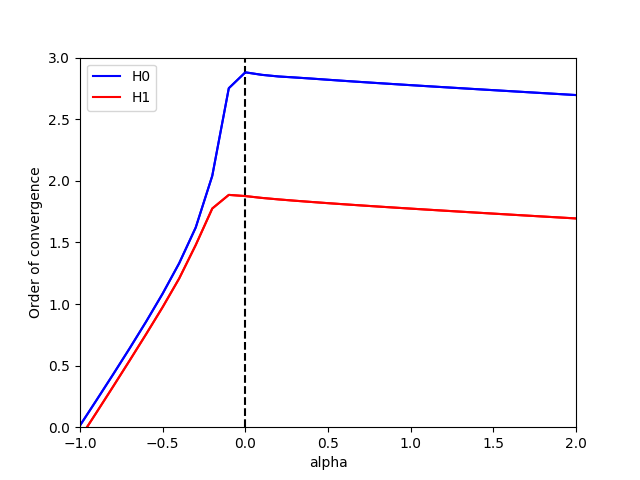
\includegraphics[width=5in]{conv.PNG}
\caption{Observed behavior of convergence order as dependent on $\alpha$, quadratic elements.}
\end{figure}

\begin{figure}[!htb]
\centering
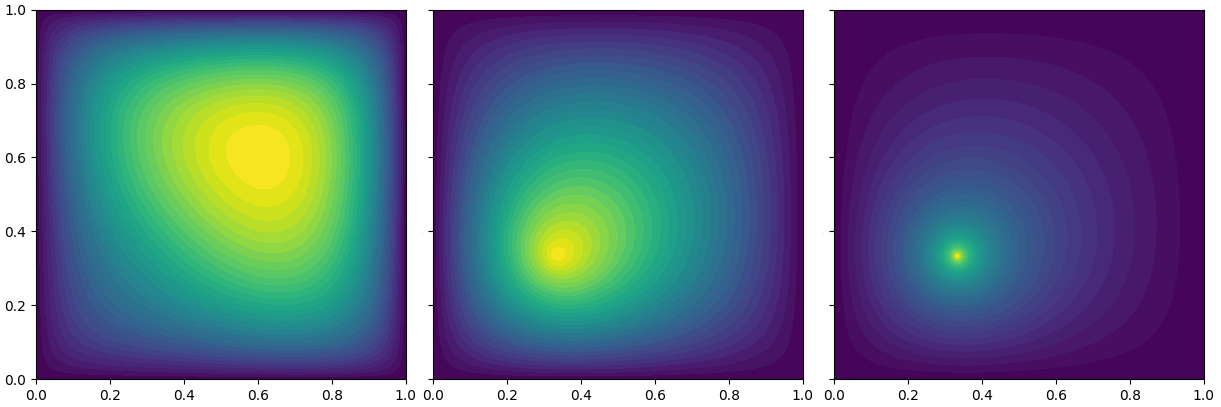
\includegraphics[width=1 \linewidth]{comp.PNG}
\caption{Change in nature of solution as $\alpha$ varies. Left to right: $\alpha =$ 0.5, -0.5, -1.}
\end{figure}

\end{document}